\documentclass[twocolumn, a4j]{jsarticle}

\usepackage{listings, jlisting, color}
\usepackage[dvipdfmx]{graphicx}
\usepackage{pdfpages}
\usepackage{amsmath}
\usepackage{mathtools}
\usepackage{multirow}
\usepackage{color}
\usepackage{ulem}
\usepackage{here}
\usepackage{wrapfig}
\usepackage[margin=20mm]{geometry}
%%図を二個横に並べるときに使用
\usepackage[hang,small,bf]{caption}
\usepackage[subrefformat=parens]{subcaption}
%%\urlを使用する際に必要
\usepackage{url}

\renewcommand{\baselinestretch}{0.78}

\setlength{\columnwidth}{5mm}

\lstset{
  basicstyle={\ttfamily},
  identifierstyle={\small},
  commentstyle={\smallitshape},
  keywordstyle={\small\bfseries},
  ndkeywordstyle={\small},
  stringstyle={\small\ttfamily},
  frame={tb},
  breaklines=true,
  columns=[l]{fullflexible},
  numbers=left,
  xrightmargin=0zw,
  xleftmargin=3zw,
  numberstyle={\scriptsize},
  stepnumber=1,
  numbersep=1zw,
  lineskip=-0.5ex
}

\makeatletter % プリアンブルで定義開始

% 表示文字列を"図"から"Figure”へ,"表"から"Table”へ
\renewcommand{\figurename}{図}
\renewcommand{\tablename}{表}

% 図,表番号を"<章番号>.<図番号>” ,"<章番号>.<表番号>” へ
\renewcommand{\thefigure}{\thesection-\arabic{figure}}
\renewcommand{\thetable}{\thesection-\arabic{table}}

% 章が進むごとに図番号をリセットする
\@addtoreset{figure}{section}
\@addtoreset{table}{section}

\makeatother % プリアンブルで定義終了

\begin{document}
\twocolumn[
  \title{
    LSIデザインコンテスト 進捗報告
    \large{\\---画像をVAEで圧縮したい---}}
  \author{222C1021 今村優希}
  \maketitle

  \section{進捗概要}
  今週は,教授から頂いた\texttt{insole\_jude\_VAE.m}のプログラムを改良し,ブロック画像でもきちんと出力がなされるかの検証を行った.
  まずは,通常の画像を白黒にし,ブロック(今回は16×16)に分割するプログラムを作成.
  そのブロックを教師データとし,1枚, 3枚, 10枚, 256枚と増加させながらテストデータがきちんと出力できているかを確認した.
  最終的に,すべてのブロックをVAEに学習させ,同じデータの入出力を確認するところまで行うことができた.
  出力されたデータから再合成した画像に関しては,精度としては良くないものの,どんな画像か判別することはできた.
]

\section{前回の振り返り}
前回は,テーマ決め,及びVivadoを用いた設計の概略を学んだ.
また,ブロック画像を入れて,きちんと動くか検証することを課題としていた.

\section{今回の実施内容}
今回は,以下のプログラムの作成,変更と出力画像の検証を行った.
\begin{itemize}
  \item 入力画像を白黒にし,ブロックに変化させるプログラム
  \\ブロックのサイズは16×16でり,使用した画像(デジコンの演習で使用した\texttt{input.bmp})では256ブロックできた.
  \item \texttt{insole\_judge\_VAE.m}の改良版
  \\及び,下記VAEの本体とforwardプログラム
  \begin{itemize}
    \item \texttt{Neuralnetwork\_VAE.m}
    \item \texttt{Neuralnetwork\_forward\_VAE.m}
  \end{itemize} 
  \item 出力した縦ベクトルからブロックに戻し,ブロックを再結合するプログラム.
\end{itemize}

\section{実験と考察}
\subsection{実験1}
\subsubsection{内容}
教師データとしてブロック1つ,テストデータとしてブロックを2つ入力した.
使用したブロックは図\ref{fig:3-1},図\ref{fig:3-2}である.
\\条件:Layer2 = 2, epoch = 100,000 
\begin{figure}[]
  \begin{minipage}[b]{0.49\columnwidth}
    \centering
    \includegraphics[width=0.9\columnwidth]{figure/block1.bmp}
    \subcaption{教師データかつテストデータ}
    \label{fig:3-1}
  \end{minipage}
  \begin{minipage}[b]{0.49\linewidth}
    \centering
    \includegraphics[width=0.9\columnwidth]{figure/block2.bmp}
    \subcaption{テストデータ}
    \label{fig:3-2}
  \end{minipage}
  \caption{実験1で使用したブロック画像}
\end{figure}

\subsubsection{結果}
VAEで学習し,教師データとテストデータどちらもVAEに通した結果が図\ref{fig:3-3-1}である.
入力データどちらも教師データの画像に似たものが出力された.
また,学習率の推移として,図\ref{fig:3-5}に示す.
\begin{figure}[]
  \begin{minipage}[b]{0.49\columnwidth}
    \centering
    
\includegraphics[width=0.9\columnwidth]{figure/archive20241219-figure102_1.png}
    \subcaption{教師データの出力結果}
    \label{fig:3-3}
  \end{minipage}
  \begin{minipage}[b]{0.49\linewidth}
    \centering
    
\includegraphics[width=0.9\columnwidth]{figure/archive20241219-figure102_2.png}
    \subcaption{テストデータの出力結果}
    \label{fig:3-4}
  \end{minipage}
  \caption{入力したブロック画像の出力結果}
  \label{fig:3-3-1}
\end{figure}
\begin{figure}
  \begin{center}
    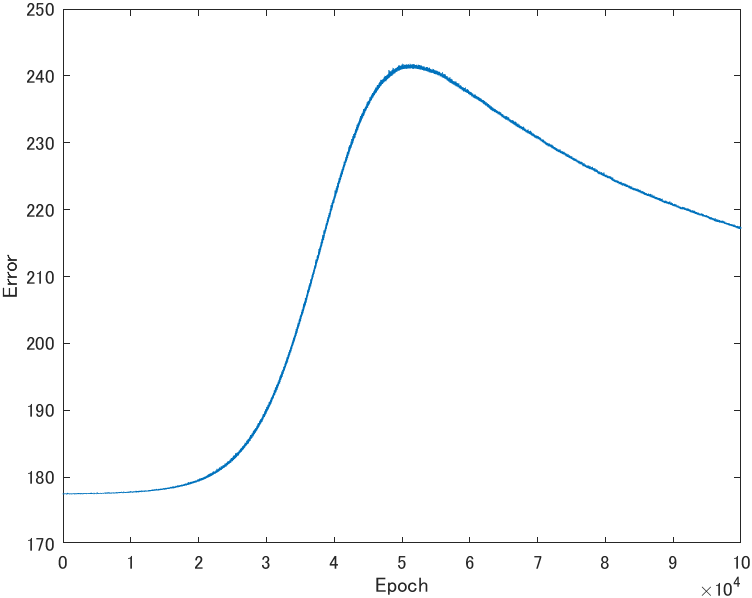
\includegraphics[width=0.9\columnwidth]{figure/archive20241219-figure3.png}
  \end{center}
  \caption{学習率の推移}
  \label{fig:3-5}
\end{figure}

\subsubsection{考察}
今回は教師データ1枚のみを学ばせたので,VAEに通したブロック2枚とも教師データに似た画像が出力されたと考えられる.

\subsection{実験2}
\subsubsection{内容}
教師画像を10枚にして実験を行った.
\\条件:Layer2 = 3, epoch = 100,000
\subsubsection{結果}
実行を行って出力画像を見ても特性等が良くわからなかった.
学習率を図\ref{fig:3-6}に表示する.
\begin{figure}[h]
  \begin{center}
    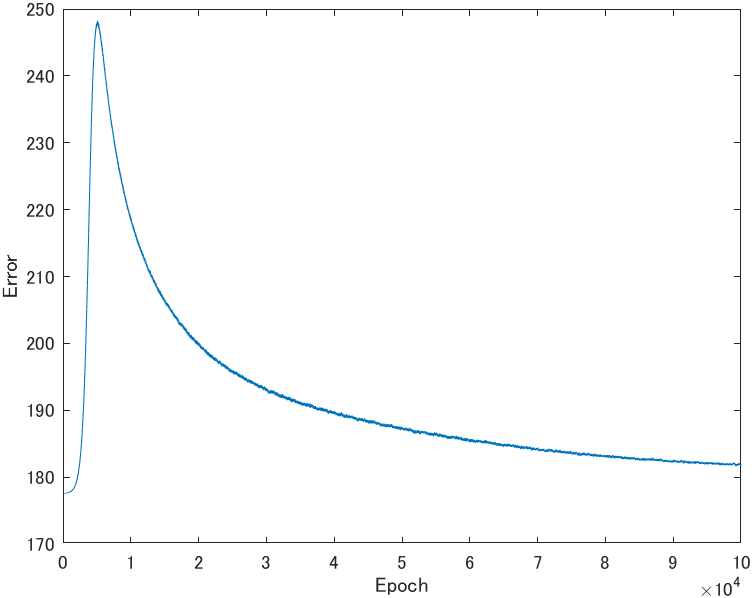
\includegraphics[width=0.9\columnwidth]{figure/archive20241219-figure3-2.png}
  \end{center}
  \caption{学習率の推移}
  \label{fig:3-6}
\end{figure}
\subsubsection{考察}
出力画像だけ見てもなんにもわからないので,もっと入力画像数を増やし,ブロックを結合させることにした.

\subsection{実験3}
\subsubsection{内容}
入力ブロック数を全てにして実験を行った.
\\条件: Layer2 = 32, epoch = 120,000

\subsubsection{結果}
出力されたブロック全てを結合して得られた画像を図\ref{fig:3-7}に示す.
ブロックノイズが鮮明に見えるが,何の画像かはわかるぐらい特徴は残っている.
また,学習率を図\ref{fig:3-8}に示す.
2枚や10枚と異なり,学習率が思ったように下がっていないのが気になる.
\begin{figure}[h]
  \begin{center}
    \includegraphics[width=0.9\columnwidth]{figure/output.bmp}
  \end{center}
  \caption{結合後の画像}
  \label{fig:3-7}
\end{figure}
\begin{figure}[h]
  \begin{center}
    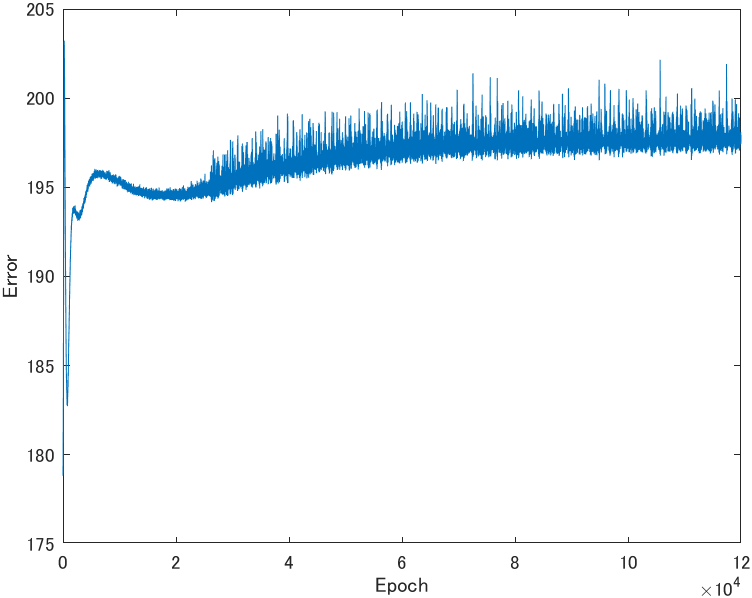
\includegraphics[width=0.9\columnwidth]{figure/archive20241218-figure3.png}
  \end{center}
  \caption{学習率の推移}
  \label{fig:3-8}
\end{figure}
\subsubsection{考察}
教師データが多すぎるため,潜在空間にうまく落とし込めていないのかもしれない.
しかし,結合後の画像を見ても分かる通り,何の画像かは判別できる状態であるから,VAEを用いた画像圧縮も可能かもしれない.

\section{課題}
\begin{itemize}
  \item 課題0\\
  元データとどのくらいの誤差があるのかの確認
  \\↑MATLABでプログラムを作成する時間がなかった
  \item 課題1\\
  ブロックノイズができるだけ消えるようなアルゴリズムの変更
  \item 課題2\\
  VAEに通して,潜在空間の情報だけでどのくらいのデータ量になっているかの検証
  \item 課題3\\
  応用として,使用したい画像を用いた画像圧縮シミュレーションを行う
  \item 課題4\\
  課題3の延長線として,VAEの特性である異常検知等を行えるかの検証
\end{itemize}

\section{今後の計画}
今月中にシミュレーションをある程度完了させたいという考えから,課題3,4にまず取り組みたいと考えている.

考えているのは,道路情報カメラ等の画像データが圧縮できるかどうかである.
すでに似たような研究がされていたので,その情報を元に自分たちでアイデアを練って行こうと思っている.
今現在考えている構想は以下の通り,
\begin{itemize}
  \item[1] 画像情報から道路の位置を把握
  \item[2] 道路部分が少しでも被っているブロックに対してVAEで学習させる
  \item[3] 実際にテストデータを用いて検証,修正を行う
\end{itemize}

  %\bibitem{1} 
\begin{thebibliography}{9}
  \bibitem{1} 山本,橋本他,"平均画像に対するVAE異常検知の適用による道路落下物検出", 人工知能学会全国大会論文集,35回, 2021, 
  \url{https://www.jstage.jst.go.jp/article/pjsai/JSAI2021/0/JSAI2021_2F1GS10f03/_article/-char/ja/}
\end{thebibliography}
\end{document}